\documentclass[aspectratio=169,10pt]{beamer}

\usepackage[utf8]{inputenc}
\usepackage[T1]{fontenc}
\usepackage[spanish]{babel}
\usepackage{lmodern}
\usepackage{graphicx}
\usepackage{booktabs}
\usepackage{tikz}
\usepackage{pgfplots}
\usetikzlibrary{arrows.meta, positioning, shapes.geometric, fit, calc}
\pgfplotsset{compat=1.18}

\definecolor{OlistNavy}{HTML}{17324D}
\definecolor{OlistTeal}{HTML}{07838B}
\definecolor{OlistOrange}{HTML}{E3943A}
\definecolor{OlistPale}{HTML}{EEF3F6}
\definecolor{OlistGray}{HTML}{526475}
\definecolor{OlistGreen}{HTML}{3A8D78}

\usetheme{Boadilla}
\setbeamercolor{normal text}{fg=OlistNavy,bg=white}
\setbeamercolor{structure}{fg=OlistTeal}
\setbeamercolor{title}{fg=OlistNavy}
\setbeamercolor{frametitle}{fg=OlistNavy,bg=white}
\setbeamercolor{block title}{fg=white,bg=OlistTeal}
\setbeamercolor{block body}{fg=OlistNavy,bg=OlistPale}
\setbeamercolor{alerted text}{fg=OlistOrange}
\setbeamertemplate{navigation symbols}{}
\setbeamertemplate{footline}{}
\setbeamersize{text margin left=7mm,text margin right=7mm}

\title{Olist | Pulso comercial}
\subtitle{Un flujo ELT incremental en Databricks Free Edition}
\author{Diego Bernales}
\date{Proyecto individual}

\tikzset{
  arrow/.style={-{Stealth[length=2.2mm]},thick,draw=OlistTeal},
  softarrow/.style={-{Stealth[length=2mm]},thick,draw=OlistGray},
  arch/.style={draw=OlistTeal,fill=OlistPale,rounded corners=2mm,
    minimum width=2.15cm,minimum height=1.38cm,align=center,
    text width=1.98cm,font=\scriptsize},
  data/.style={draw=OlistNavy,fill=white,rounded corners=2mm,
    minimum width=3.3cm,minimum height=1.18cm,align=center,
    text width=3.08cm,font=\small},
  control/.style={draw=OlistOrange,fill=white,rounded corners=2mm,
    minimum width=3.1cm,minimum height=.82cm,align=center,
    text width=2.88cm,font=\scriptsize},
  dim/.style={draw=OlistTeal,fill=OlistPale,rounded corners=2mm,
    minimum width=2.7cm,minimum height=1.1cm,align=center,
    text width=2.48cm,font=\scriptsize},
  fact/.style={draw=OlistNavy,fill=OlistNavy,text=white,rounded corners=2mm,
    minimum width=3.35cm,minimum height=1.55cm,align=center,
    text width=3.08cm,font=\scriptsize}
}

\begin{document}

% 1 | 0:20
\begingroup
\setbeamercolor{background canvas}{bg=OlistPale}
\begin{frame}[plain]
  \vspace*{1.1cm}
  \hspace*{1.2cm}\begin{minipage}{.78\textwidth}
    {\color{OlistTeal}\rule{1.4cm}{3pt}\par}
    \vspace{.4cm}
    {\usebeamerfont{title}\color{OlistNavy}\LARGE\bfseries Olist | Pulso comercial\par}
    \vspace{.3cm}
    {\large Un flujo ELT incremental en Databricks Free Edition\par}
    \vspace{1.0cm}
    {\color{OlistGray}\large Diego Bernales\par}
    \vspace{.2cm}
    {\color{OlistGray}\small Proyecto individual | Ingeniería de datos\par}
    \vfill
    \begin{beamercolorbox}[rounded=true,sep=.65em,wd=\linewidth]{block body}
      \color{OlistTeal}\small Del archivo CSV a una decisión comercial, con trazabilidad de punta a punta
    \end{beamercolorbox}
  \end{minipage}
\end{frame}
\endgroup

% 2 | 0:45
\begin{frame}{El caso de negocio}
  \begin{beamercolorbox}[rounded=true,sep=.65em,wd=\linewidth]{block body}
    \textbf{Supuesto académico:} el equipo comercial de Olist solicita una vista
    sencilla para decidir dónde enfocar el catálogo y entender cómo evolucionan
    las ventas y el despacho de pedidos.
  \end{beamercolorbox}
  \vspace{.65em}
  \begin{columns}[T,onlytextwidth]
    \column{.46\textwidth}
      \begin{block}{¿Qué categorías lideran el importe?}
        Ayuda a priorizar la revisión del surtido y las acciones comerciales.
      \end{block}
      \begin{block}{¿Cómo cambia cada mes?}
        Da contexto temporal para observar subidas, caídas y meses sin ventas.
      \end{block}
    \column{.46\textwidth}
      \begin{block}{¿Qué UF tiene mayor ticket?}
        Permite comparar mercados regionales sin confundir volumen con valor medio.
      \end{block}
      \begin{block}{¿Cómo avanzan los pedidos?}
        Aporta una lectura operativa de entregas, cancelaciones y despacho.
      \end{block}
  \end{columns}
  \vspace{.2em}
  {\centering\small\color{OlistGray}
  Filtros comunes: mes, UF del cliente y estado del pedido.\par}
\end{frame}

% 3 | 0:40
\begin{frame}{Datos, alcance y definición de importe}
  \begin{columns}[T,onlytextwidth]
    \column{.49\textwidth}
      \begin{beamercolorbox}[rounded=true,sep=.45em,wd=\linewidth]{block body}
        \small\textbf{Fuente pública}\enspace Brazilian E-Commerce by Olist\par
        8 tipos de CSV | histórico de sep. 2016 a sep. 2018\par
        {\tiny\color{OlistGray}Kaggle | licencia CC BY-NC-SA 4.0}
      \end{beamercolorbox}
    \column{.49\textwidth}
      \begin{beamercolorbox}[rounded=true,sep=.45em,wd=\linewidth]{block body}
        \small\textbf{Importe}\enspace precio del artículo + flete de su línea.\par
        No representa el total pagado por el pedido.
      \end{beamercolorbox}
  \end{columns}
  \vspace{.25em}
  \begin{tikzpicture}
        \begin{axis}[
          width=\linewidth,height=4.45cm,
          xmin=0,xmax=27,ymin=0,ymax=1.6,
          xtick={0,4,8,12,16,20,24,27},
          xticklabels={sep-16,ene-17,may-17,sep-17,ene-18,may-18,sep-18,dic-18},
          ytick={0,0.5,1.0,1.5},
          yticklabels={{0},{0,5},{1,0},{1,5}},
          tick label style={font=\tiny},
          label style={font=\scriptsize},
          axis line style={OlistGray!45},
          grid=major,grid style={OlistPale},
          ylabel={Importe mensual (R\$ millones)},
          xlabel={Mes de compra},
          legend style={font=\tiny,draw=none,fill=white,at={(0.98,0.98)},anchor=north east},
          clip=false
        ]
          \addplot[OlistNavy,very thick,mark=none] coordinates {
            (0,0.000355) (1,0.056809) (2,0) (3,0.000020) (4,0.137188)
            (5,0.286281) (6,0.432049) (7,0.412422) (8,0.586191)
            (9,0.502963) (10,0.584972) (11,0.668205) (12,0.720399)
            (13,0.769312) (14,1.179144) (15,0.863547) (16,1.107302)
            (17,0.986909) (18,1.155127) (19,1.159698) (20,1.149782)
            (21,1.022677) (22,1.058728) (23,1.003308) (24,0.000166)
            (25,0) (26,1.32) (27,1.48)
          };
          \addlegendentry{Serie mensual Gold}
          \addplot[OlistOrange,only marks,mark=square*,mark size=2.5pt]
            coordinates {(26,1.32) (27,1.48)};
          \addlegendentry{Demo sintética}
        \end{axis}
  \end{tikzpicture}
  \vspace{-.05em}
  {\centering\scriptsize\color{OlistGray}
  Serie histórica hasta sep. 2018; noviembre y diciembre son una extensión sintética.\par}
\end{frame}

% 4 | 0:50
\begin{frame}{Arquitectura ELT en Databricks}
  \centering
  \begin{tikzpicture}[node distance=3mm and 2mm]
    \node[arch] (source) {Fuente\par\textbf{Kaggle}\par 8 CSV originales};
    \node[arch,right=of source] (raw) {Volumen Raw\par\texttt{inbox/} a \texttt{olist/}\par carpeta por tipo de CSV};
    \node[arch,right=of raw] (bronze) {Bronze\par Delta crudo\par Auto Loader\par CDF habilitado};
    \node[arch,right=of bronze] (silver) {Silver\par limpieza y reglas\par CDF habilitado};
    \node[arch,right=of silver] (gold) {Gold\par modelo estrella\par hechos + dimensiones};
    \node[arch,right=of gold] (bi) {Power BI\par conexión Import\par análisis comercial};
    \draw[arrow] (source) -- (raw);
    \draw[arrow] (raw) -- (bronze);
    \draw[arrow] (bronze) -- (silver);
    \draw[arrow] (silver) -- (gold);
    \draw[arrow] (gold) -- (bi);

    \node[control,below=8mm of bronze] (deployer)
      {Workflow Deployer\par ejecuta DDL al desplegar el bundle};
    \node[control,right=5mm of deployer] (schedule)
      {Job ELT semanal\par Raw $\rightarrow$ Bronze $\rightarrow$ Silver $\rightarrow$ Gold};
  \end{tikzpicture}

  \vspace{.7em}
  \begin{beamercolorbox}[rounded=true,sep=.5em,wd=\linewidth]{block body}
    \centering\small
    Unity Catalog \texttt{olist\_dev}: volúmenes y watermarks en \texttt{control};
    tablas Delta en \texttt{bronze}, \texttt{silver} y \texttt{gold}.
  \end{beamercolorbox}
\end{frame}

% 5 | 0:30
\begin{frame}{Orquestación y decisiones incrementales}
  \centering
  \begin{tikzpicture}[node distance=5mm and 4mm]
    \node[data] (raw) {\textbf{Raw}\par clasifica el CSV y valida su hash};
    \node[data,right=of raw] (bronze) {\textbf{Bronze}\par Auto Loader de la tabla afectada};
    \node[data,right=of bronze] (silver) {\textbf{Silver}\par CDF Bronze + watermark};
    \node[data,right=of silver] (gold) {\textbf{Gold}\par CDF Silver + MERGE idempotente};
    \draw[arrow] (raw) -- (bronze);
    \draw[arrow] (bronze) -- (silver);
    \draw[arrow] (silver) -- (gold);
  \end{tikzpicture}

  \vspace{.35em}
  \begin{columns}[T,onlytextwidth]
    \column{.47\textwidth}
      \begin{block}{Cambios}
        \small
        \begin{itemize}\setlength\itemsep{.25em}
          \item Checkpoint independiente por tabla Bronze.
          \item Watermark CDF y \texttt{MERGE} idempotente por clave.
        \end{itemize}
      \end{block}
    \column{.47\textwidth}
      \begin{block}{Ejecución}
        \small
        \begin{itemize}\setlength\itemsep{.25em}
          \item Sin novedades: salida temprana con log claro.
          \item Silver y Gold retoman cambios pendientes desde su watermark.
        \end{itemize}
      \end{block}
  \end{columns}
  \vspace{.3em}
  {\centering\scriptsize\color{OlistGray}
  Beneficio: procesar solo los cambios y reintentar sin duplicar resultados.\par}
\end{frame}

% 6 | 0:50
\begin{frame}{Bronze: Auto Loader aislado por tipo de archivo}
  \centering
  \begin{tikzpicture}[node distance=5mm and 4mm]
    \node[data] (folder) {\textbf{Carpeta Raw}\par\scriptsize
      \texttt{.../olist/order\_items/}};
    \node[data,right=of folder] (stream) {\textbf{Estado propio}\par\scriptsize
      esquema + checkpoint\par\texttt{.../bronze/v2/}\par\texttt{brz\_order\_items/}};
    \node[data,right=of stream] (table) {\textbf{Tabla Delta}\par\scriptsize
      \texttt{olist\_dev.bronze.}\par\texttt{brz\_order\_items}\par CDF habilitado};
    \draw[arrow] (folder) -- (stream);
    \draw[arrow] (stream) -- (table);
  \end{tikzpicture}

  \vspace{.45em}
  \begin{beamercolorbox}[rounded=true,sep=.55em,wd=\linewidth]{block body}
    \small
    \textbf{Cómo decide qué leer.} Las ocho subcarpetas tienen un patrón de nombre,
    ubicación de esquema y checkpoint propios. Auto Loader usa \texttt{cloudFiles}
    con \texttt{availableNow}: procesa los archivos pendientes y termina.
  \end{beamercolorbox}
  \vspace{.3em}
  \begin{beamercolorbox}[rounded=true,sep=.45em,wd=\linewidth]{block body}
    \centering\small Si llega solo \texttt{order\_items}, se activa \texttt{brz\_order\_items};
    los otros siete flujos quedan intactos.
  \end{beamercolorbox}
  \vspace{.2em}
  {\centering\tiny\color{OlistGray}
  Checkpoint del ejemplo: \texttt{/Volumes/olist\_dev/control/olist\_state/autoloader/bronze/v2/brz\_order\_items/checkpoint}.\par}
\end{frame}

% 7 | 0:55
\begin{frame}{Silver: calidad, normalización y deduplicación}
  \begin{columns}[T,onlytextwidth]
    \column{.51\textwidth}
      \begin{block}{Reglas de limpieza}
        \small
        \begin{itemize}\setlength\itemsep{.25em}
          \item Recorte, \texttt{try\_cast} y estandarización de columnas (\texttt{lenght} $\rightarrow$ \texttt{length}).
          \item Valores categóricos a minúsculas; UF a mayúsculas.
          \item Se descartan filas sin campos obligatorios y valores negativos donde no aplican.
          \item \texttt{review\_score} debe estar entre 1 y 5.
        \end{itemize}
      \end{block}
      \vspace{.2em}
      \begin{beamercolorbox}[rounded=true,sep=.4em,wd=\linewidth]{block body}
        \scriptsize\textbf{Para qué:} descartar registros incompletos o inválidos y
        unificar formatos para que las uniones y filtros sean consistentes.
      \end{beamercolorbox}
    \column{.45\textwidth}
      \begin{block}{Deduplicación por clave de negocio}
        \scriptsize
        \begin{tabular}{@{}ll@{}}
          \textbf{Tabla} & \textbf{Clave}\\
          pedidos & \texttt{order\_id}\\
          artículos & \texttt{order\_id + order\_item\_id}\\
          clientes & \texttt{customer\_id}\\
          productos & \texttt{product\_id}\\
          pagos & \texttt{order\_id + payment\_sequential}\\
          reseñas & \texttt{review\_id + order\_id}\\
          vendedores & \texttt{seller\_id}\\
          categorías & \texttt{product\_category\_name}\\
        \end{tabular}
      \end{block}
      \vspace{.2em}
      \begin{beamercolorbox}[rounded=true,sep=.4em,wd=\linewidth]{block body}
        \scriptsize En CDF conserva el último \texttt{insert}/\texttt{update\_postimage}
        por clave antes del \texttt{MERGE}; evita varias escrituras para la misma entidad.
      \end{beamercolorbox}
  \end{columns}
\end{frame}

% 8 | 0:50
\begin{frame}{Watermarks CDF: avance y recuperación}
  \begin{columns}[T,onlytextwidth]
    \column{.49\textwidth}
      \begin{beamercolorbox}[rounded=true,sep=.45em,wd=\linewidth]{block body}
        \centering\small\textbf{\texttt{olist\_dev.control.cdf\_watermarks}}\par
        \vspace{.2em}
        \scriptsize\texttt{source\_table} : STRING\par
        \texttt{target\_table} : STRING\par
        \texttt{last\_processed\_commit\_version} : BIGINT\par
        \texttt{last\_processed\_commit\_timestamp} : TIMESTAMP\par
        \texttt{updated\_at} : TIMESTAMP\par
        \vspace{.15em}
        \tiny Una fila por fuente Bronze; por ejemplo, \texttt{brz\_orders} $\rightarrow$ \texttt{slv\_orders}.
      \end{beamercolorbox}
    \column{.49\textwidth}
      \begin{beamercolorbox}[rounded=true,sep=.45em,wd=\linewidth]{block body}
        \centering\small\textbf{\texttt{olist\_dev.control.gold\_cdf\_watermarks}}\par
        \vspace{.2em}
        \scriptsize\texttt{source\_table} : STRING\par
        \texttt{target\_table} : STRING\par
        \texttt{last\_processed\_commit\_version} : BIGINT\par
        \texttt{last\_processed\_commit\_timestamp} : TIMESTAMP\par
        \texttt{updated\_at} : TIMESTAMP\par
        \vspace{.15em}
        \tiny Una fila por fuente Silver; por ejemplo, \texttt{slv\_order\_items} $\rightarrow$ \texttt{fct\_order\_items}.
      \end{beamercolorbox}
  \end{columns}
  \vspace{.4em}
  \begin{tikzpicture}[node distance=6mm and 5mm]
    \node[control] (read) {Leer desde watermark + 1 hasta la última versión};
    \node[control,right=of read] (apply) {Conservar post-images y aplicar \texttt{MERGE}};
    \node[control,right=of apply] (save) {Guardar versión y timestamp tras éxito};
    \draw[arrow] (read) -- (apply);
    \draw[arrow] (apply) -- (save);
  \end{tikzpicture}
  \vspace{.3em}
  \begin{beamercolorbox}[rounded=true,sep=.4em,wd=\linewidth]{block body}
    \centering\scriptsize La clave de control es \texttt{source\_table}. Tras un fallo se retoma
    desde la última versión confirmada. CDF tiene retención finita: hay que mantenerlo al día.
  \end{beamercolorbox}
\end{frame}

% 9 | 0:35
\begin{frame}{Gold: modelo estrella para análisis}
  \begin{columns}[T,onlytextwidth]
  \column{.72\textwidth}
      \centering
      \begin{tikzpicture}[node distance=7mm and 9mm]
        \node[fact] (f) {\textbf{fct\_order\_items}\par grano: una fila por artículo del pedido\par
          importe, precio, flete, cantidad y claves};
        \node[dim,above=of f] (date) {\textbf{dim\_date}\par fecha, mes, trimestre y año};
        \node[dim,left=of f] (customer) {\textbf{dim\_customer}\par cliente y UF};
        \node[dim,right=of f] (product) {\textbf{dim\_product}\par producto y categoría};
        \node[dim,below=of f] (seller) {\textbf{dim\_seller}\par vendedor};
        \draw[softarrow] (date) -- (f);
        \draw[softarrow] (customer) -- (f);
        \draw[softarrow] (product) -- (f);
        \draw[softarrow] (seller) -- (f);
      \end{tikzpicture}
    \column{.29\textwidth}
      \begin{block}{Medidas del reporte}
        \small
        \textbf{Importe}\par
        precio + flete por línea\par\vspace{.35em}
        \textbf{Ticket promedio}\par
        importe / pedidos distintos\par\vspace{.35em}
        \textbf{Pedido}\par
        \scriptsize Clave degenerada:\par\texttt{order\_id}
      \end{block}
  \end{columns}
\end{frame}

% 10 | 1:10
\begin{frame}{Power BI responde preguntas complementarias}
  \centering
  \small\color{OlistGray}
  ¿Cuánto importa se registra? ¿Qué categorías y mercados destacan? ¿Cómo están los pedidos?
  \vspace{.35em}
  \begin{columns}[T,onlytextwidth]
    \column{.5\textwidth}
      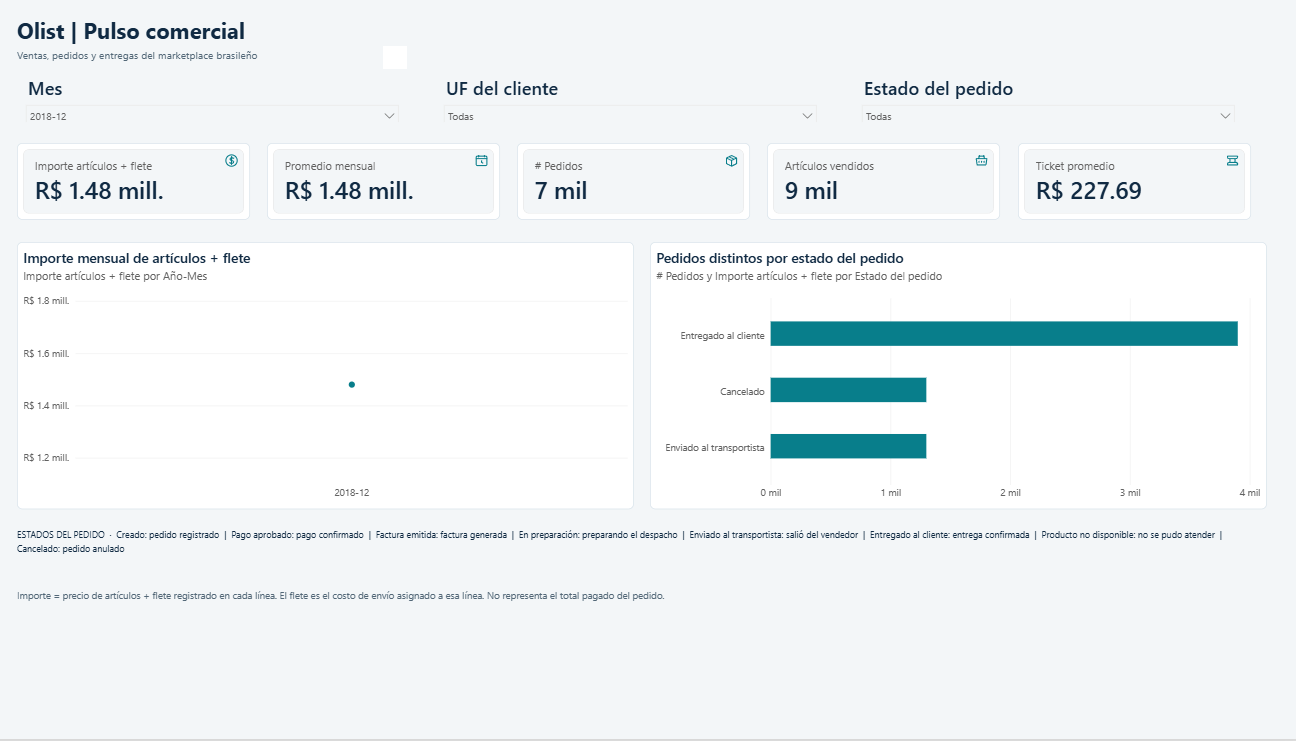
\includegraphics[width=\linewidth,height=4.0cm,keepaspectratio]{assets/pulso_comercial_201812.png}
      \vspace{.1em}
      {\scriptsize\textbf{01 | Pulso comercial}}
    \column{.5\textwidth}
      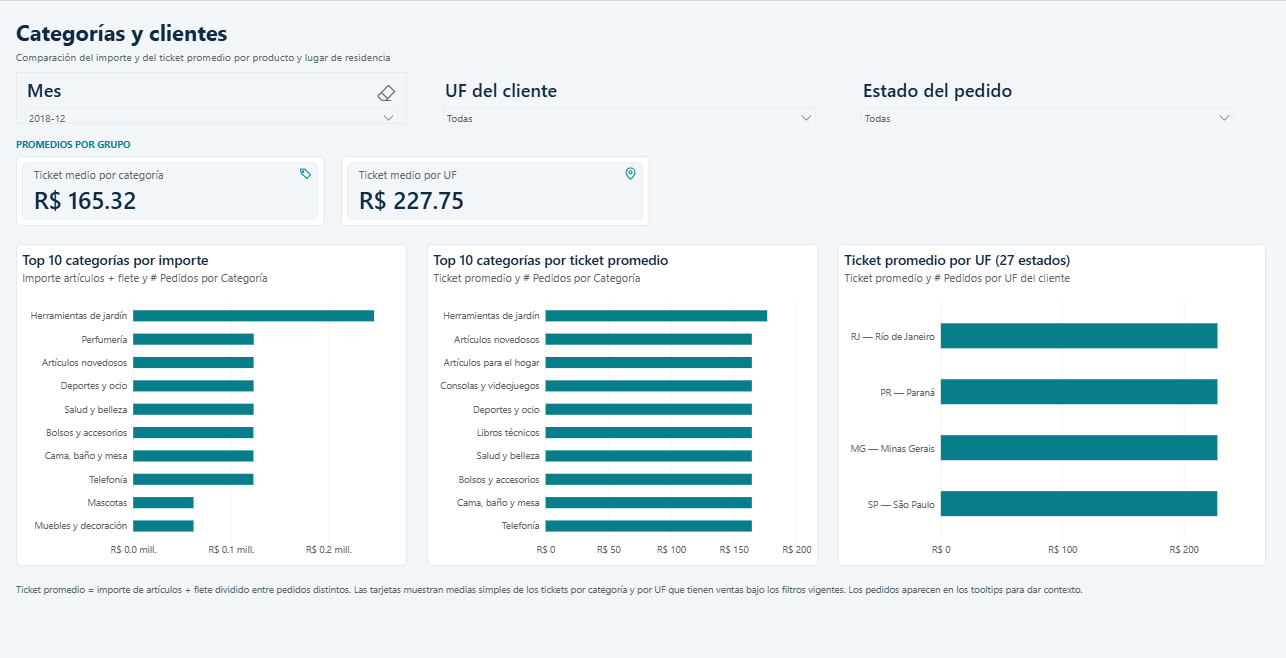
\includegraphics[width=\linewidth,height=4.0cm,keepaspectratio]{assets/categorias_clientes_201812.png}
      \vspace{.1em}
      {\scriptsize\textbf{02 | Categorías y clientes}}
  \end{columns}
  \vspace{.35em}
  \begin{beamercolorbox}[rounded=true,sep=.35em,wd=\linewidth]{block body}
    \centering\scriptsize Capturas con filtro \texttt{2018-12}; el lote mostrado es sintético.
    La tarjeta de pedidos redondea 6.500 a ``7 mil''; el conteo exacto de Gold es 6.500.
  \end{beamercolorbox}
\end{frame}

% 11 | 0:25 + demo posterior
\begin{frame}{Validación de punta a punta}
  \centering
  \small
  \begin{tabular}{@{}lrrr@{}}
    \toprule
    \textbf{Alcance} & \textbf{Pedidos} & \textbf{Artículos} & \textbf{Importe} \\
    \midrule
    Histórico público & 98.666 & 112.650 & R\$15.843.553,24 \\
    Demo sintética nov.--dic. & 12.500 & 17.000 & R\$2.800.000,00 \\
    \textbf{Acumulado} & \textbf{111.166} & \textbf{129.650} & \textbf{R\$18.643.553,24} \\
    \bottomrule
  \end{tabular}
  \vspace{.25em}
  \vspace{.15em}
  \makebox[\linewidth][c]{\scriptsize Seis categorías con mayor importe acumulado hasta dic. 2018 (R\$ millones)}
  \vspace{.15em}
  \centering
  \begin{tikzpicture}
    \begin{axis}[
      xbar,width=.78\linewidth,height=3.6cm,
      xmin=0,xmax=1.8,
      ytick={0,1,2,3,4,5},
      yticklabels={Salud y belleza,Cama y baño,Deportes y ocio,Relojes y regalos,Computación,Herramientas de jardín},
      y dir=reverse,
      yticklabel style={font=\scriptsize,text width=2.8cm,align=right},
      xtick={0,0.5,1.0,1.5},
      xticklabels={0,0.5,1.0,1.5},
      tick label style={font=\tiny},
      xlabel={Importe (R\$ millones)},
      label style={font=\scriptsize},
      axis line style={OlistGray!45},
      grid=major,grid style={OlistPale},
      nodes near coords={\pgfmathprintnumber[fixed,precision=2]{\pgfplotspointmeta}},
      nodes near coords style={font=\scriptsize,text=white,anchor=east,xshift=-1pt},
    ]
      \addplot[fill=OlistTeal,draw=OlistTeal] coordinates {
        (1.6746,0) (1.4748,1) (1.3899,2) (1.3055,3) (1.0593,4) (1.0511,5)
      };
    \end{axis}
  \end{tikzpicture}
  \vspace{-.15em}
  \begin{beamercolorbox}[rounded=true,sep=.35em,wd=\linewidth]{block body}
    \centering\scriptsize Reejecución: 0 archivos copiados; Bronze, Silver y Gold sin cambios.
    La demo en vivo usará el lote sintético 2019-01 y un refresco manual de Power BI.
  \end{beamercolorbox}
\end{frame}

\end{document}
